\subsection{Part B: Real-CV validation}
\label{sec:method-partb}

\subsubsection{Marker target and its as-printed geometry}

The target uses the original ArUco dictionary (5$\times$5 payload) with the dock's marker set: two 155.64~mm markers (IDs 201, 202), one 77.82~mm (301), four 46.69~mm (302 to 305) and two 36.96~mm (401, 402), printed across three A4 sheets taped to a rigid panel. The as-printed geometry was estimated from the data rather than assumed: a size-weighted least-squares fit over all nine markers (residuals under 0.4~mm) shows the sheets were printed at 95.9\% of nominal scale, so the analysis uses the measured black-square sides (149.4, 74.7, 44.4 and 35.6~mm) throughout. The fit is corroborated independently by the 201-to-202 baseline, which matches two butted A4 pages plus millimetres of tape gap only under the corrected scale; using nominal sizes would silently inflate every derived range by 4.1\%. The as-measured layout is shown in Figure~\ref{fig:board}.

\begin{figure}[H]
    \centering
    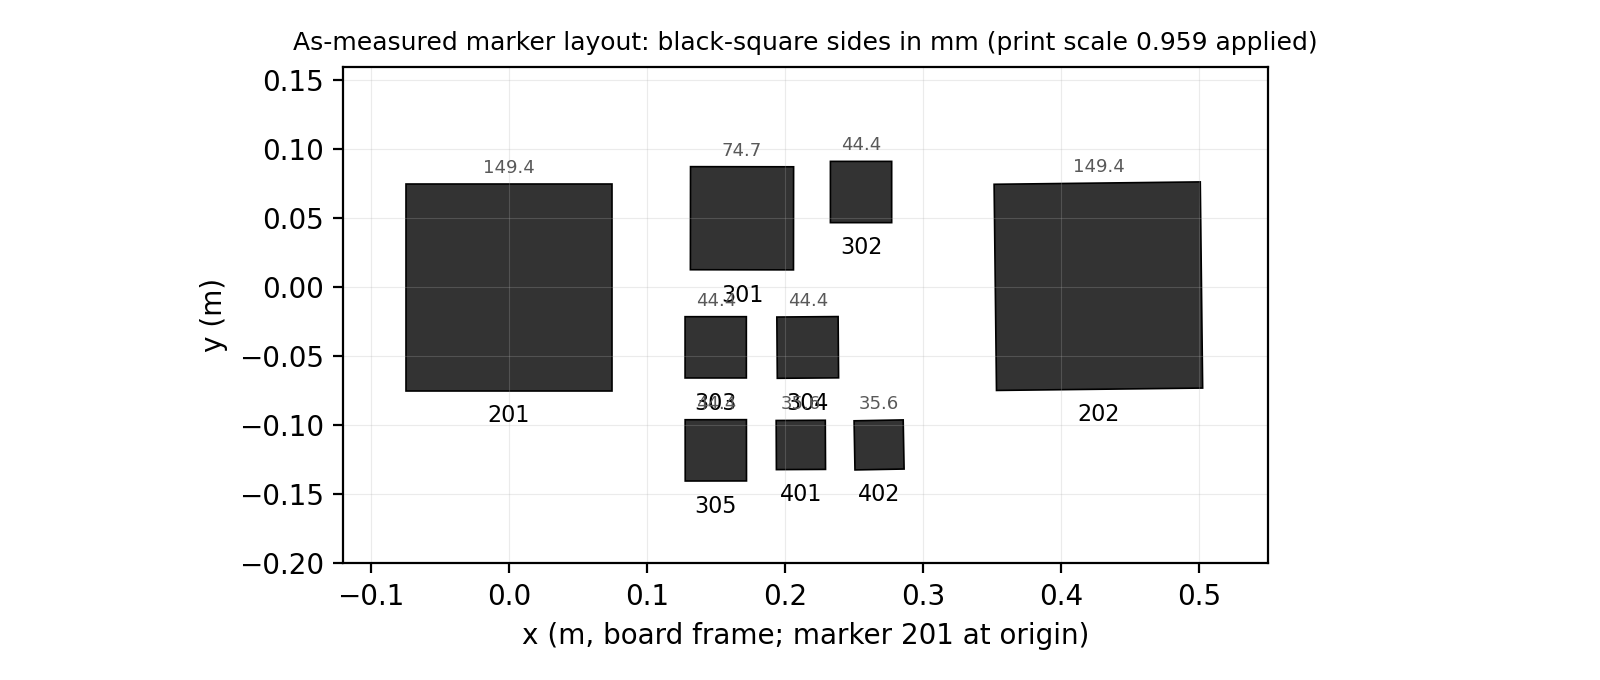
\includegraphics[width=0.85\textwidth]{Figures/board_layout.png}
    \caption{As-measured marker layout in the board frame, positions and
    black-square sides estimated from the data with the 0.959 print scale
    applied. The four size groups placed at a common range are the
    marker-size lever of the experiment.}
    \label{fig:board}
\end{figure}

\subsubsection{Capture setup}

Data was captured in a single pool session with a ZED stereo camera, of which only the left, rectified stream was recorded (960$\times$540 at nominal 15~Hz), giving a monocular ArUco problem; images, camera info and the ZED IMU were logged. Two runs were recorded: an on-axis walk-back (677 frames at an effective 2.5~Hz over 271~s) and an oblique walk-back from roughly 4~m of lateral offset (737 frames over 85~s, with about 42\% of frames dropped in bursts by disk bandwidth; the two runs are therefore analysed separately and never pooled). The vehicle was hand-held and paced backwards from the board to beyond the detection limit, with a yaw turn at each step.

Camera intrinsics are the shipped in-air factory rectification ($f_x{=}f_y{=}797.5$, zero distortion on the rectified stream). The in-water validity of this choice was tested by a joint bundle adjustment over 1400 marker observations in 317 frames, solving for underwater focal lengths, the coplanar board layout and per-frame poses with scale pinned by the ruler-measured marker sizes: the aspect ratio solves to $f_y/f_x = 0.996$ and the isotropic optimum is only 1.9\% better than the in-air value, while the flat-port refraction correction of $1.333\times$ is rejected outright (44\% worse residual). The shipped intrinsics are therefore used unchanged, and all metric ranges carry an approximately $\pm$10\% scale uncertainty from the focal length, which dominates the error budget. For this reason the primary independent variable throughout Part~B is the calibration-free \emph{apparent marker size in pixels}; metric range is derived and reported with its uncertainty.

\subsubsection{Experiment design}

The two walk-backs sweep range continuously from about 0.6~m to beyond the detection limit, and marker size is swept \emph{by construction}: four size groups (149.4 down to 35.6~mm, a 4.2$\times$ lever) are present on the board simultaneously, so every frame samples all sizes at a common range and water condition. Viewing angle was not controlled: the on-axis run has a median marker incidence of 13$^\circ$ and the oblique run 58$^\circ$, two disconnected regimes confounded with range and marker size, so no detection-versus-angle curve is reported.

No external ground truth exists (no tape or survey range, and vehicle odometry was not recorded); scale is anchored solely by the ruler-measured marker sizes and attitude solely by an IMU gravity check. Detection is scored per marker-frame trial against apparent-size bins with a minimum of ten trials per bin and Wilson confidence intervals (2551 trials on-axis, 950 oblique). Maximum detection range is established uncensored: the on-axis walk continued for a further 79~s (about 3~m) beyond the last detection with zero detections, and two independent end-of-run estimates (walk-back rate extrapolation and board apparent width in the final frame) agree at 7.8 to 8.1~m, so range limits below are detection failures, not end-of-data artefacts.

\subsubsection{Turbidity measurement and synthetic degradation}

Water attenuation was measured photometrically from the target itself, without dosing or a turbidity meter. A black patch (marker border) and a white patch (surrounding sheet) at the same range share an identical veiling-light term in the image formation model $I = J e^{-\beta d} + B(1 - e^{-\beta d})$, so their difference is free of $B$: $\mathrm{contrast}(d) = (J_w - J_b)\,e^{-\beta d}$, and $\beta$ is a straight-line fit in log space. Two corrections proved load-bearing: an instrument-response correction $k$(apparent~px), measured at fixed range so it is independent of $\beta$, without which small (hence distant-looking) markers read up to 18\% low and the bias imitates attenuation; and per-marker intercepts, since the three sheets sit under different local lighting. The underlying image formation model is the standard attenuation-plus-veiling form \cite{jaffe1990computer}.

Higher turbidity than the pool's was synthesised by re-attenuating each real frame in place: $I' = B + (I - B)\,e^{-\Delta\beta\, d(x)}$ per channel and per pixel, with the per-pixel range $d(x)$ taken from the board-plane pose and $\Delta\beta = m\,\beta$ for multipliers $m \in \{0, 0.25, 0.5, 1, 1.5, 2, 3, 4, 6, 8\}$, where $m{=}0$ reproduces the real frame. Results are reported against total optical depth $\tau = (1{+}m)\,\beta d$ rather than named water types: range enters the model only as the product $\beta d$, so any uniform scale error in $d$ is absorbed into $\beta$, making the $\tau$ axis immune to the $\pm$10\% range uncertainty and portable across waters and cameras. The synthesis adds no scattering blur, so any benefit a contrast-enhancing preprocessor shows on synthesised frames is an upper bound. The full chain is summarised in Figure~\ref{fig:turbpipe}.

\begin{figure}[H]
\centering
\begin{tikzpicture}[font=\scriptsize, >={Stealth[length=2mm]},
  box/.style={draw, rounded corners=1pt, align=center, minimum height=9mm, inner sep=3pt}]
  \node[box] (frame) {frame};
  \node[box, right=6mm of frame] (warp) {canonical\\marker warp};
  \node[box, right=6mm of warp] (patch) {black ring /\\white surround};
  \node[box, right=6mm of patch] (contrast) {$B$-free contrast\\$(J_w{-}J_b)e^{-\beta d}$};
  \node[box, right=6mm of contrast] (corr) {$k(\mathrm{px})$ +\\fixed effects};
  \node[box, right=6mm of corr] (beta) {$\beta$ per\\channel};
  \node[box, below=8mm of beta] (synth) {re-attenuate:\\$I' = B + (I{-}B)e^{-m\beta d(x)}$};
  \node[box, left=6mm of synth] (sweep) {detection sweep\\(2551 trials $\times$ 10 levels)};
  \node[box, left=6mm of sweep] (env) {envelope:\\rate(px, $\tau$), sizing rule};
  \draw[->] (frame) -- (warp);
  \draw[->] (warp) -- (patch);
  \draw[->] (patch) -- (contrast);
  \draw[->] (contrast) -- (corr);
  \draw[->] (corr) -- (beta);
  \draw[->] (beta) -- (synth);
  \draw[->] (synth) -- (sweep);
  \draw[->] (sweep) -- (env);
\end{tikzpicture}
\caption{Turbidity processing: the top row measures the water's
attenuation from the target itself via the veiling-free contrast; the
bottom row stresses the same real frames to higher optical depth and maps
the detection envelope.}
\label{fig:turbpipe}
\end{figure}

\subsubsection{Detection pipeline and metrics}

Detection uses OpenCV~4.10 with the current \texttt{ArucoDetector} API, subpixel corner refinement, and \texttt{adaptiveThreshConstant} lowered from the default 7 to 3, the best of a grid over $\{3, 5, 7\}$ scored at the highest synthesised turbidity (selected without a holdout, so its reported rate is an optimistic bound). Single-marker pose, the quantity under test, uses planar PnP (IPPE square); the reference for self-consistency is a multi-marker board PnP computed leave-one-out, with the marker under test excluded from its own reference. Off-board IDs are deliberately not filtered so the misidentification rate remains measurable. Reported metrics are detection rate per apparent-size bin and per derived-range bin, uncensored maximum detection range per marker, single-marker translation and rotation deviation from the board reference (self-consistency, not accuracy, since no ground truth exists), misidentification rate, and an IMU gravity check as the sole camera-independent attitude validation.
